

\section{Signaler och anrop}
\subsection{Landsprefix}

Här är inte alla länder med utan de vanligaste som körs från Sverige.

\begin{center}
	\begin{footnotesize}
		\begin{longtable}{lll}
			\caption{Utvalda landsprefix} \\
			\textbf{Land}                 & \textbf{DXCC}  & \textbf{Prefixserier}                             \\ \hline
			Belgien                       & ON             & ONA--OTZ                                          \\
			Canada                        & VE             & CYA--CZZ, VAA--VGZ, VOA--VOZ, VXA--VYZ, XJA--XOZ  \\
			Frankrike                     & F              & FAA--FZZ, HWA--HWZ, THA--THZ, TKA--TKZ, TMA--TMZ, \\
			                              &                & TOA--TQZ, TVA--TXZ                                \\
			Frankr. särsk.                & FG FH FK       &                                                   \\
			                              & FM, FO, FP, FR &                                                   \\
			                              & FS, FT, FW, FY &                                                   \\
			Förenta Staterna              & K              & AAA--ALZ, KAA--KZZ, NAA--NZZ, WAA--WZZ            \\
			Grekland                      & SV             & J4A--J4Z, SVA--SVZ                                \\
			Italien                       & I              & IAA--IZZ                                          \\
			Japan                         & JA             & 7JA--7NZ, 8JA--8NZ, JAA--JSZ                      \\
			Kroatien                      & 9A             & 9AA--9AZ                                          \\
			Nederländerna                 & PA             & PAA--PLZ                                          \\
			Polen                         & SP             & 3ZA--3ZZ, HFA--HFZ, SNA--SRZ                      \\
			Rumänien                      & YO             & YOA--YRZ                                          \\
			Ryssland (Eur.)               & UA1 3 4 5 6 7  & RAA--RZZ, UAA-UIZ                                 \\
			Ryssland (Asi.)               & UA8 9 0        & RAA--RZZ, UAA-UIZ                                 \\
			Schweiz                       & HB             & HBA--HBZ HEA--HEZ                                 \\
			Spanien                       & EA             & AMA--AOZ, EAA--EHZ                                \\
			Storbritt. England            & G, 2E, M       & 2AA--2ZZ, GAA--GZZ, MAA--MZZ, VPA--VQZ,           \\
			                              &                & VSA--VSZ,ZBA--ZJZ, ZNA--ZOZ, ZQA--ZQZ             \\
			Storbritt. Skottland          & GM, 2M, MM     &                                                   \\
			Storbritt. Övrigt             & VP2, VP6, VP8  &                                                   \\
			                              & VP9, VQ9, ZB   &                                                   \\
			Sverige                       & SM             & 7SA--7SZ, 8SA--8SZ, SAA--SMZ                      \\
			Tyskland                      & DL             & DAA--DRZ, Y2A--Y9Z                                \\
			Ukraina                       & UT             & EMA--EOZ, URA--UZA                                \\
			Ungern                        & HA             & HAA--HAZ, HGA--HGZ                                \\
			Österrike                     & OE             & OEA--OEZ\\
		\end{longtable}
	\end{footnotesize}
\end{center}

\subsection{Svenska signaler}

Svenska signaler förekommer inom ett antal prefix. Enligt ITU disponerar Sverige förljande signalserier: 7SA--7SZ samt 8SA--8SZ och vidare de mer kända SAA--SMZ. Dessa har används till varierande ändamål, exempelvis har flyget signaler i serien SE-AAA--ZZZ. Polisen har tidigare använt signaler i serien SHA plus fyra siffror, detta är nu ersatt med nytt system i.o.m. RAKEL. Räddningstjänsten använde SDA med fyra siffror. Signaler som 7SA + 4 siffror används för mindre yrkesbåtar SC + 4 siffror för fritidsbåtar.

Amatörradion använder ett antal signaler, de viktigaste är:

\begin{tabular}{ll}
	SM & Amatörradiosignal utdelad av PTS (nya signaler tilldelas ej i serien)               \\
	SA & Amatörradiosignal tilldelad av SSA                                                  \\
	SK & Klubbsignaler (som regel tvåställiga efter distriktsiffran)                         \\
	   & numera tilldelas även klubbar SA-signaler som är tvåställiga efter distriktssiffran \\
	SL & Militära signaler (som regel två- eller treställiga efter distriktsiffran)
\end{tabular}

Dessa signaler följs av en \textit{distriktsiffra} se särskilt avsnitt och sedan 2-ställiga eller 3-ställiga bokstavskombinationer som är den personliga signalen. Exempel är SM0UEI som är min egen signal, distriktsiffran är 0 dvs hemmavarande i Stockholms län. Ett annat exempel kan vara SK5JV tidigare Fagersta amatörradioklubb.

Repeatrar som tillhör klubbar får ofta signal efter klubben med tillägg /R för repeater.

Det finns numera även ett stort antal signaler som är tillfälliga eller knutna till särskilda event, exempelvis scoutverksamhet som ibland sänder amatörradio och särskilda forskningsfartyg, flyg- och rymdfart mm.

Som suffix används följande:

\begin{tabular}{ll}
	/M  & Mobil (rörlig) sändaramatör, även portabel \\
	/MM & Mobil till sjöss (mobil maritime)          \\
	/AM & Mobil i luften (aeromobile)                \\
	/P  & Portabel (för stunden uppsatt station)     \\
	/R  & Repeaterstation
\end{tabular}

\subsection{Svenska distrikten}

Sverige delas in i följande distrikt efter sina län:

\begin{table}[h]
	\centering
\begin{tabular}{cl}
	\textbf{Distrikt} & \textbf{Län}                                     \\ \hline %\endhead
	      0        & Stockholm                                        \\
	      1        & Gotland                                          \\
	      2        & Västerbotten, Norrbotten                         \\
	      3        & Gävleborg, Jämtland, Västernorrland              \\
	      4        & Örebro, Värmland, Dalarna                        \\
	      5        & Östergötland, Södermanland, Västmanland, Uppsala \\
	      6        & Halland, Västra götaland                         \\
	      7        & Skåne, Blekinge, Kronoberg, Jönköping, Kalmar    \\
	      8        & Speciella stationer utanför landets gränser
\end{tabular}
\caption{Distriktssiffor i Sverige}
\end{table}

\subsubsection{Karta över svenska amatörradiodistrikt}

\begin{wrapfigure}{R}{15cm}
	\centering
	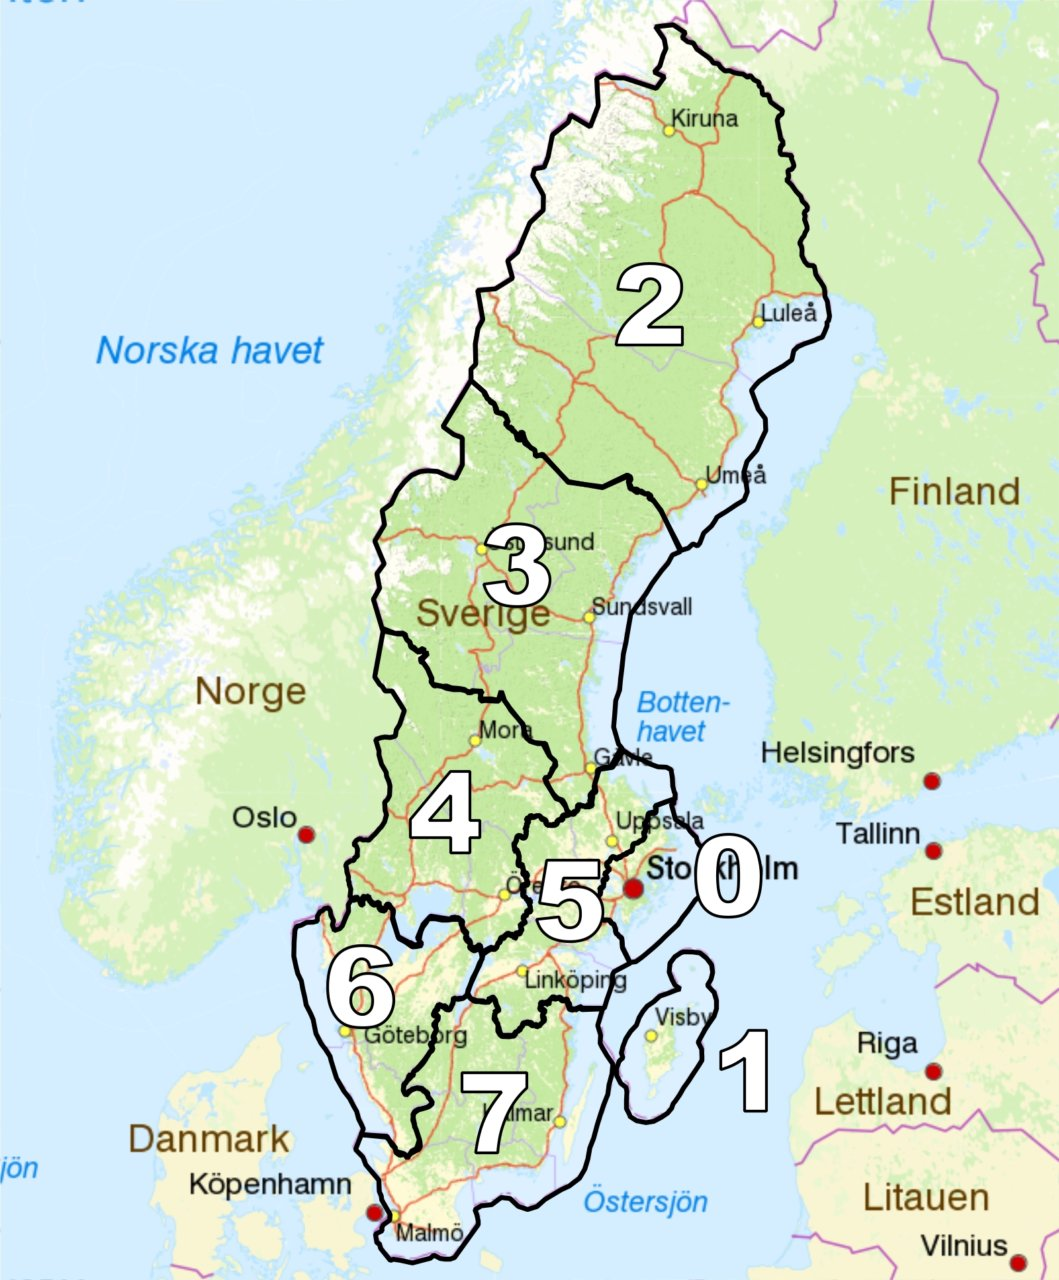
\includegraphics[width=15cm]{pic/sm-distrikt-stor}
	\label{fig:sm-distrikt}
	\caption{Svenska distrikt, karta med tillståpnd från \href{https://SSA.SE}{ssa.se}}
\end{wrapfigure}

Distrikten förekommer som siffra i utdelade anropssignaler. Radioamatörer 
byter inte distriktsiffra under resa i annat distrikt, i stället används 
suffix (tillägg efter ordinarie signal) som t.ex. /M för mobil. Ofta uppger 
man "SM0UEI mobilt i SM3-land" (SM0UEI/3/M) ibland (SM0UEI/3M) för att 
påvisa att man befinner sig utanför ordinarie distrikt.

En radioamatör kan byta sin distriktsiffra om den sänder från ett
annat distrikt än sitt hemmavarande. Man kan också göra ett tillägg
med /n där n är den siffra för det distrikt man befinner sig i. En
stockholmsamatör som befinner sig i Gävleborgs län kan alltså antingen
använda SM3UEI eller SM0UEI/3 även med tillägget M för mobil och P för
portabel om man så önskar.

Det unika för en radioamatörs signal är alltså prefixet + suffixet,
som exempel är identifieraren för SM0UEI prefixet SM och suffixet UEI
eftersom distriktsiffran kan ändra sig. 

\clearpage


\section{Terminologi och trafik}

\subsection{Bokstaveringsalfabetet (Svenska)}

\begin{table}[H]
	\centering
\begin{longtable}{cl|cl|cl }
	A & Adam   & O & Olof    & 1 & Ett        \\
	B & Bertil & P & Petter  & 2 & Tvåa       \\
	C & Cesar  & Q & Qvintus & 3 & Trea       \\
	D & David  & R & Rudolf  & 4 & Fyra       \\
	E & Erik   & S & Sigurd  & 5 & Femma      \\
	F & Filip  & T & Tore    & 6 & Sexa       \\
	G & Gustav & U & Urban   & 7 & Sju        \\
	H & Helge  & V & Viktor  & 8 & Åtta       \\
	I & Ivar   & W & Wilhelm & 9 & Nia        \\
	J & Johan  & X & Xerxes  & 0 & Nolla      \\
	K & Kalle  & Y & Yngve   & . & Punkt      \\
	L & Ludvig & Z & Zäta    & , & Komma      \\
	M & Martin & Å & Åke     & - & Minus      \\
	N & Niklas & Ä & Ärlig   & + & Plus       \\
	  &        & Ö & Östen   &   & Mellanslag \\
\end{longtable}
\caption{Svenska bokstaveringsalfabetet}
\end{table}

\subsection{Bokstaveringsalfabetet (Internationella)}
\begin{table}[H]
\centering
\begin{tabular}{cl|cl|cl}
	A & Alfa     &  P   & Papa       & 0 & Zero    \\
	B & Bravo    &  Q   & Quebec     & 1 & One     \\
	C & Charlie  &  R   & Romeo      & 2 & Two     \\
	D & Delta    &  S   & Sierra     & 3 & Tree    \\
	E & Echo     &  T   & Tango      & 4 & Fower   \\
	F & Foxtrot  &  U   & Uniform    & 5 & Fife    \\
	G & Golf     &  V   & Victor     & 6 & Six     \\
	H & Hotel    &  W   & Whiskey    & 7 & Seven   \\
	I & India    &  X   & X-ray      & 8 & Ait     \\
	J & Juliet   &  Y   & Yankee     & 9 & Niner   \\
	K & Kilo     &  Z   & Zulu       & . & Stop    \\
	L & Lima     & Å/AA & Alfa-Alfa  & , & Decimal \\
	M & Mike     & Ä/AE & Alfa-Echo  & - & Minus   \\
	N & November & Ö/OE & Oscar-Echo & + & Plus    \\
	O & Oscar    &      &            &   & Space   \\
\end{tabular}
\caption{Internationella bokstaveringsalfabetet (ITU-alfabetet)}
\end{table}

\subsection{Q-koder}
I tabellen listas några av de vanligast förekommande Q-koderna på amatörradiobanden. 
Det finns förstås många fler koder men detta anses som de vanligaste.

\begin{longtable}{ll}
	\textbf{Kod} & \textbf{Fråga / Svar}                                                         \\ \hline 
	\endhead
	\caption{Q-koder}\\    
\endlastfoot
	QRA & Vad heter er station?                                                \\
	    & Vår station heter ...                                                \\ \hline
	QRB & Hur långt bort från min station befinner ni er?                      \\
	    & Avståndet mellan oss är ungefär ...                                  \\ \hline
	QRG & Kan ni ange min exakta frekvens?                                     \\
	    & Er exakta frekvens är ... (MHz/kHz)                                  \\ \hline
	QRH & Varierar min frekvens/våglängd?                                      \\
	    & Er frekvens/våglängd varierar.                                       \\ \hline
	QRI & Hur är min sändningston (CW)?                                        \\
	    & Er sändningston är 1--God, 2--Varierande, 3--Dålig                   \\ \hline
	QRK & Vilken uppfattbarhet har mina signaler?                              \\
	    & Uppfattbarheten hos dina signaler är:                                \\
	    & 1--Dålig, 2--Bristfällig, 3--Ganska god, 4--God, 5--Utmärkt          \\ \hline
	QRL & Är ni upptagen?                                                      \\
	    & Jag är upptagen med ... (namn/signal) stör ej.                       \\ \hline
	QRM & Är ni störd av annan station?                                        \\
	    & Störningarna är:                                                     \\
	    & 1--Obef., 2--Svaga, 3--Måttliga, 4--Starka, 5--Mycket starka         \\ \hline
	QRN & Besväras ni av atmosfäriska störningar?                              \\
	    & Störningarna är:                                                     \\
	    & 1--Obef., 2--Svaga, 3--Måttliga, 4--Starka, 5--Mycket starka         \\ \hline
	QRO & Kan jag (ska jag) öka sändareffekten?                                \\
	    & Öka sändareffekten.                                                  \\ \hline
	QRP & Kan jag (ska jag) minska sändareffekten?                             \\
	    & Minska sändareffekten.                                               \\ \hline
	QRQ & Kan jag (får jag) öka sändningshastigheten?                          \\
	    & Öka sändningshastigheten.                                            \\ \hline
	QRS & Kan jag (skall jag) sända långsammare?                               \\
	    & Sänd långsammare.                                                    \\ \hline
	QRT & Skall jag avbryta sändningen?                                        \\
	    & Avbryt sändningen                                                    \\ \hline
	QRU & Har ni något till mig?                                               \\
	    & Jag har inget till er. Se även QTC.                                  \\ \hline
	QRV & Är ni redo?                                                          \\
	    & Jag är redo.                                                         \\ \hline
	QRX & När anropar ni mig härnäst?                                          \\
	    & Jag anropar er kl ... (på ... MHz/kHz)                               \\ \hline
	QRZ & Vem anropar mig?                                                     \\
	    & Ni anropas av ... (på ... MHz/kHz).                                  \\ \hline
	QSA & Vilken styrka har mina signaler?                                     \\
	    & Era signaler är:                                                     \\
	    & 1--Ej uppf., 2--Svaga, 3--Ganska starka, 4--Starka, 5--Mycket starka \\ \hline
	QSB & Svajar styrkan på mina signaler?                                     \\
	    & Styrkan på era signaler svajar.                                      \\ \hline
	QSK & Kan du höra mig mellan dina tecken och får jag avbryta dig?          \\
	    & Jag kan höra dig mellan mina tecken och du får avbryta.              \\ \hline
	QSL & Kan ni ge mig kvittens?                                              \\
	    & Jag kvitterar.                                                       \\ \hline
	QSO & Ha ni förbindelse med ... eller ... (förmedlat)?                     \\
	    & Jag har förbindelse med ... (via ...)                                \\ \hline
	QST & Har tidigare använts som allmänt anrop men ersatts av CQ             \\ \hline
	QSY & Skall jag övergå till att sända på annan frekvens?                   \\
	    & Gå över till att sända på annan frekvens (eller ... kHz/MHz).        \\ \hline
	QTC & Hur många telegram har ni att sända?                                 \\
	    & Jag har ... telegram till dig (eller ...).                           \\ \hline
	QTH & Vilken är er geografiska position?                                   \\
	    & Min geografiska position är ...                                      \\ \hline
	QTR & Kan ni ge mig rätt tid?                                              \\
	    & Rätt tid är ...                                                      \\ 
\end{longtable}

\subsection{Lokator}

Lokator (Maidenhead locator) är ett praktiskt sätt att tala om sin ungefärliga position genom att ange endast sex stycken tecken. En lokator kan t.ex. se ut som JO89VK vilket täcker in nordvästa Järfälla. Det finns många verktyg för att räkna på lokator där ute, det är bra att känna sin egen. Det finns appar för detta till telefonerna som både kan räkna på bäring, distans mellan två rutor och dessutom via telefonens GPS bestämma vilken lokator du för närvarande befinner dig i.

Första paret dela in jorden i 18x18 fält, dvs 20 grader per fält longitud och 10 grader per fält latitud. Varje sådant fält delas sedan in i 10x10 rutor som numreras 0-9 på vardera axeln. Dessa i sin tur delas sedan in i 24x24 smårutor som då får storleksordningen 2.5 grader latitud och 5 grader long. vardera.

\subsection{Uppträdande}

När vi kör amatörradio finns det ett antal saker att tänka på som har att göra med hur vi beter oss mot varandra på banden. Se detta som en guide till hur man bör uppträda på banden.

En radioamatör måste vara \textbf{tolerant}. Vi delar frekvenser med många andra personer, en del av dem kommer inte ha samma uppfattning som du själv har om saker och ting. Här gäller det att vara tolerant, förstående och framför allt inte bli upprörd över personer som kanske inte beter sig som du önskade att de betedde sig.

Radioamatörer är \emph{aldrig ensamma på banden} helt oavsett om någon svarar på ditt allmänna anrop eller ej så finns det i det närmaste \textbf{garanterat någon som lyssnar}. 

Tänk på vad du säger och att du undviker diskutera ämnen som kan verka \textbf{upprörande} eller \textbf{stötande}. Ämnen som bör undvikas är \textbf{religion} och livs\-å\-skå\-d\-ni\-ng, \textbf{politisk} ideologi, \textbf{ekonomiska} eller \textbf{sociala} frågor m.m. där motparter kan ha starka åsikter som inte nödvändigtvis stämmer med dina egna. Radion är inte ett agitationsrum för sådana frågor.

\textbf{Svordomar}, \textbf{könsord} och liknande undviker vi helt. Språket skall vara vårdat men behöver inte vara strikt. Tänk på att din motpart är inte den enda som lyssnar utan det finns \textit{andra amatörer som lyssnar}, icke-amatörer som lyssnar, myndigheter som lyssnar och så vidare.

Ha \textbf{förståelse} för att andra kanske inte har dina egna detaljkunskaper, professionalism med mera. Agera \textbf{ödmjukt} gentemot andra människor på banden.

Blir du ändå upprörd, undvik att \emph{agera på det} över huvud taget. Sänd inte över annans sändning, s.k. ''gummitumme'', eller stör på annat vis för du är upprörd. Avsluta hellre QSO:t, byt frekvens eller återkom lite senare när du lugnat ned dig. Tänk på att \textit{de flesta konflikter orsakas av okunskap eller brist på förståelse}. \textbf{Agera vuxet} i sådana situationer och jobba för att \textbf{de-eskalera} situationen.

En skicklig amatör \textit{lyssnar mycket innan sändning}. Vi anropar på ett korrekt sätt och avslutar på ett korrekt sätt. Vi försöker uppge våra respektive signaler på ett \emph{tydligt och läsligt sätt}, i dag finns det en tendens att sluddra över signalerna framför allt på 2m och 70cm banden, gör inte det. Tydlighet är en vinning i sig. 

När någon ny i ringen inträder, räkna upp de deltagande signalerna så att personen tydligt får en bild av alla som är med och vem som är på turen före och efter hen.

Vi pratar inte \textbf{nedvärderande} om personer varesig de är andra amatörer eller ej, eller en viss grupp av personer. Vi undviker \textbf{sexuella anspelningar} och vitsar ''\textbf{under bältet}'' liksom allt för \textbf{personliga detaljer}. Amatörradion är främst för \textbf{tekniska diskussioner} av rent \textbf{privat natur} eller av \textbf{allmänt intresse för hobbyn}, tester och prov med mera.

Undvik väldigt \textbf{långa sändningspass}. Ibland händer det saker hos dina motstationer som att de får ett viktigt telefonsamtal eller måste springa ut i köket för katten har rivit ner något, ett barn ramlar eller annat som gör att man måste kvickt lämna radion. Att \textbf{långprata} i sådana lägen gör det svårt att tala om ''QRX --- jag måste ta hand om en sak, anropar dig igen om 5 min.''. Enstaka gånger kanske man behöver förklara något lite längre men gör det till en vana att lämna luckor så ofta som möjligt.

\textbf{Nödtrafik har alltid prioritet} och måste respekteras på alla
frekvenser.

\subsection{Repeatrar}

Repeatrars syfte är främst att förlänga kommunikationen från mobila och portabla amatörsändare. Samtal mellan fasta stationer förekommer men om ni hör varandra på direkten, övergå gärna till en simplex-frekvens i stället för att belägga repeatern.

Lämna luckor mellan er när ni växlar station som sänder. Gör det möjligt för andra att ''breaka-in'' särskilt om ert QSO fortsätter under längre tid. Ta hänsyn till att andra kanske vill använda repeatern för att nå personer som de inte kan nå annars. Hänsyn åt båda hållen förutsätts här. 

Repeatern är en begränsad resurs. Det är inte okay att lägga beslag på den under långa perioder när andra kanske behöver den, var ödmjuk inför att någon driver repeatern och har satt upp den i första hand för att supporta mobila stationer.

Nödtrafik har alltid prioritet.

\subsection{QSO}

Konsten att genomföra ett radiosamtal (QSO) i olika sammanhang. Ofta
blir folk nervösa i början för hur detta går till. Man säger sin
signal och motstationens i fel ordning eller liknande.

Man börjar alltid med motstationens signal. Det bör fallas naturligt
att ropa så och man avslutar anropet med sin egen signal så att
motstationen dels vet vem som anropar men också andra hör. Kanske vill
en annan station ha ett utbyte med dig om du inte får svar från den
tilltänkta.

Ett radiosamtal består som regel av tre delar. Först sker ett anrop, när kontakt etablerats utväxlas ett antal meddelande (dialog) och när man är klarar avslutas samtalet. Dessa tre delar är ganska standard. Man följer detta ganska strikt t.ex. på kortvågen där telefoni oftast innebär SSB. Anledningen är enkel, det går inte höra när någon släpper sändtangenten eller bara är tyst och tänker.

När man kör FM över repeatrar på VHF/UHF är det inte lika vanligt att man både öppnar och avslutar varje sändning med motparten och sin egen signal. Men man skall regelbundet upprepa signalerna och i praktiken är det lämpligt att göra kanske var femte minut eller oftare.

\subsubsection{Anropet}

Ett anrop kan se ut ungefär såhär:

\begin{tabular}{ll}
	Station & Meddelande                            \\ \hline
	SMØUEI  & SAØMAD från SMØUEI, SAØMAD kom.       \\
	SAØMAD  & SMØUEI från SAØMAD, jag lyssnar, kom.
\end{tabular}

Därefter övergår radiosamtalet i dialog eller meddelandesändning.

\subsubsection{Allmänt anrop} 

Används när man inte ropar på någon särskild motstation utan önskar samtal med vem som helst. På svenska använder man ofta just orden ''allmänt anrop'' medan på engelska är det vanligare att man uttalar CQ (seek you). Ett allmänt androp kan se ut såhär:

-- Allmänt anrop, allmänt anrop, allmänt anrop från SM0UEI SM0UEI SM0UEI kallar allmänt anrop och lyssnar.

Eller på engelska:

-- CQ CQ CQ this is SMØUEI calling CQ CQ CQ and standing by.

\subsubsection{Meddelandesändning}

-- SA0MAD från SM0UEI, tack för svaret. Din signal är 59 hos mig, mitt QTH är JO89WA och namnet är Anders. SA0MAD från SM0UEI kom.

-- SM0UEI från SA0MAD, tack för rapporten. Din signal är 57 hos mig, jag befinner mig i JO89VK men kommer under kvällen byta QTH. Jag kommer då vara QRV på 3663 kHz. QSL? SM0UEI från SA0MAD.

-- SA0MAD från SM0UEI, QSL på det, QRX 19.30 på frekvens 3663 kHz. 

\subsubsection{Avslutning}

-- SA0MAD från SM0UEI, tack för rapport och vi hörs senare, 73, slut kom

-- SM0UEI från SA0MAD, 73 tillbaka, klart slut.

\subsubsection{Pile-up och tävling}

Ibland kan det bli väldigt många motstationer samtidigt som ropar. Nu gäller det att spetsa öronen! Först gäller det att sålla. Rara signaler från långtbortistan ger mer poäng i en contest som regel eller från länder du inte kört osv beroende på regler. Försök att sålla med ''du som sänder från Florida'' eller ''VK7 kom igen'' osv till det är en station kvar. Kör den snabbt, ropa CQ igen och börja sålla igen. Stationer du hör signalen på kör du direkt.

Direkt när det uppstår en pile-up är det effektivt att köra split. Dvs du lyssnar 5--10\,kHz upp eller ned från den frekvens du sänder på. Det gör det lättare för dig att behålla kommandot under pile-up. Ligger du och sänder i ett frekvensområde som är särskilt ägnat för DX är det smart att lägga Rx-frekvensen strax utanför. Det undviker att man stökar ned i DX-bandet.

Kör du split skall du säga det efter varje sändning. "CQ CQ CQ de Sierra Mike Zero Uniform Echo India listening 5 up" exempelvis. På CW bör en split vara minst 2 kHz och på SSB bör den vara minst 5 kHz ännu hellre 10 kHz. Tänk på att när du startar din split måste du kolla så att båda frekvenserna är ok. Låt inte din pile-up sprida ut sig för mycket även om det är kanske enklare för dig så är risken stor att den stör någon annan. 

Kör korta QSO. Utbyt snabbt den information som behövs och ta sedan nästa. Ha förståelse för att det kan bli krockar i en pile-up. När du hör en partiell signal eller station du vill prata med håll fast vid den. Om du har svårt att läsa den be den repetera tills ni är klara. Genom att du är auktoriteten på frekvensen kommer pile-up:en att lugna ned sig och vänta på sin tur. Om du ''hattar omkring'' är risken att all radiodisciplin far ut genom fönstret.

Ofta är det 1 kHz upp som gäller vid CW och digitala trafiksätt.
Du vill försöka få tag i Södra Shetlandsöarna, ett mycket ovanligt DX, som har en stor pile up och ropar på 14.195 MHz

\begin{tabular}{lrl}
	Station & Frekvens & Meddelande                     \\ \hline
	VP8SSI  &   14.195 & QRZ VP8SSI  5 to 15 UP         \\
	SMØUEI  &   14.203 & SM0UEI                         \\
	VP8SSI  &   14.195 & SM0UEI 59                      \\
	SMØUEI  &   14.203 & 59 thank you                   \\
	VP8SSI  &   14.195 & Thanks. QRZ VP8SSI 5 to 15 up.
\end{tabular}

Du kommer troligtvis att behöva upprepa din anropssignal flera gånger, men lyssna efter varje gång du ropat så att du hör vem han svarar. Svarar han inte dig så får du vänta tills han ropar något som indikerar att han avslutat kontakten. Exempelvis: Thanks, VP8SSI eller VP8SSI 5 to 15 up.

Du deltar i en tävling där man skall ange singnalrapport och löpnumret från start av tävlingenpå den kontakt du har. Du har hitintills kontaktat 30 stationer i tävlingen. Du har hittat en ledig frekvens och ropar CQ.

\begin{tabular}{ll}
	Station & Meddelande                       \\ \hline
	SMØUEI  & CQ contest SM0UEI SM0UEI contest \\
	ON3XYZ  & ON3XYZ                           \\
	SMØUEI  & ON3XYZ you are 59 031            \\
	ON3XYZ  & Thanks 031 you are 59 044        \\
	SMØUEI  & 44 Thanks. QRZ SM0UEI
\end{tabular}

Notera att både när man jagar DX och när man deltar i tävlingar så ger man och får man signalrapporten 59 om man kör foni och 599 telegrafi åtminstone i internationella tävlingar för att minska risken för fel. Får du en annan signalrapport än 59 eller 599 i en tävling så är det viktigt du anger korrekt i din logg. I mer lokala tester som NAC och SAC förekommer det att man ger korrekta signalrapporter, alltså efter hur väl man hörs.

Om du försöker nå en motstation med pile-up var uppmärksam på dennes sändningar och vänta på din tur. Tala gärna om signal och var du sänder från men släpp sedan fram andra. Tänk på hur du själv skulle vilja att en pile-up på din egen station skulle vilja agera. Den gyllene regeln är också alltid lyssna först --- sänd sedan!


\newpage

\section{Teknik}

\subsection{Amatörradiocertifikat}

Amatörradio har en lång historia och sträcker sig tillbaka till
radions barndom. Rent formellt så var det i USA i slutet av 1890-talet
som radioamatörer började sända telegram till varandra med den teknik
som fanns till buds då. Det blev mycket populärt bland elingenjörer
och andra teknikintresserade och runt 1910 började man få problem med
interferens och störningar ochg beslutade sig för att formalisera det
hela. Olika restriktioner infördes men i och med detta regelverk fick
vi också vissa krav på kunskaper för att operera radiosändare.

\subsubsection{Amatörradiocertifikat HAREC}

Om det fulla amatörradiocertifikatet är ett certifikat som är utformat
efter de principer som anges i HAREC T/R 61-02, Harmonised Amateur
Radio Examination Certificate, Vilnius 2004, uppdaterad 2014 och 2016.

Detta är ett ganska omfattande dokument och i Sverige så har vi t.ex.
KonCEPT-boken som används för ubildning av nya radioamatörer, den kan
laddas ned som PDF från ssa.se eller beställas som papperbok i deras
webshop. För att bli radioamatör behöver man svara tillräckligt många
rätt på två stycken delprov, ett teknikprov som avhandlar elektriska
kretsar, radioteknik, sändare och mottagare, vågutbredning,
eletromagnetiska fält, grundläggande matematik och fysik som är
tillämplig, viss komponentlära, förståelse för störningar och att bli
störd, filter och antenner mm. Det andra provet är ett prov över
reglementet som tillämpas, både lagar och författningar som reglerar
amatörradio men även saker som mer praktiska som exempelvis
bokstaveringsalfabetet och Q-koder mm.

Ett godkänt sådant prov ger möjlighet att operera som radioamatör på
en stor mängd olika frekvensband, alla de som i Sverige är utmärkta
som amatörradioband.

\subsubsection{Amatörradiocertifikat insteg}
\label{sec:instegscertifikat}

Instegscertifikatet är ett förenklat teknikprov men ungefär samma prov
vad gäller reglementen osv. Det förenklade teknikprovet innebär dock
en del begränsningar eftersom instegsamatören inte kan ges riktigt
samma förtroende att sända på alla frekvenser. Exempelvis har man
därmed begränsat de frekvensband som får användas till sådana som är
exklusiva för amatörradio i Sverige.

Konskapskraven i Sverige skall motsvara det som finns i ''ECC Report 89'': \\
\url{https://docdb.cept.org/download/409}. 

PTS förväntas delegera examineringen till SSA och deras utsedda provförrättare 
och en särskild utbildningbok för instegscertet håller på att tas fram just 
nu och ska snart gå till tryck (Mars 2025).

Tyvärr fick inte SSA gehör för sin remiss att även öppna 70 cm bandet 
för instegscertifikat. Bandet är inte länge ett exklusivt amatörband 
men vi delar det med lågeffektssändare för fjärrstyrning mm och det
bör inte finnas hinder då fullcertare får sända med 200\,W i bandet och
kan söka högeffektstillstånd på upp till 1\,kW.

Radioamatörer med instegscertifikat tilldelas anropssignaler i serien SH 
som även tidigare använts för noviser. Vid uppgradering till fullt cert
får man i stället en signal i SA-serien är tanken.

\subsubsection{Amatörradioband för instegscertifikat}

\begin{table}[H]
\centering
\begin{tabular}{rrlr}
	\textbf{Frekvens} & \textbf{Våglängd} & \textbf{Notiser}               & \textbf{Max Effekt} \\ \hline
	            7 MHz &          40 meter &                                &           25\,W PEP \\
	           14 MHz &          20 meter & 25\,W PEP                      &                     \\
	           21 MHz &          15 meter &                                &           25\,W PEP \\
	           28 MHz &          20 meter & Liknande utbredning som 27 MHz &           25\,W PEP \\
	           50 MHz &           6 meter &                                &           25\,W PEP \\ \hline
	          144 MHz &           2 meter &                                &           25\,W ERP
\end{tabular}
\caption{Amatörradioband i sverige upp till 70 cm}
\end{table}

50\,MHz är egentligen ett VHF-band men räknas ofta till kortvåg (HF) 
då de flesta amatörradiostationer för kortvåg omfattar även 6\,m-bandet.

Myndigheterna har gett instegscertare tillträde till amatörradioband
som är exklusiva för amatörradio vilket innebär att ett antal populära
band inte finns med. Arbete fortsätter på att försöka tillföra även 70
cm bandet (432--438 MHz) till de band som är tillåtna för
instegsamatörer men det har inte kommit med i denna utgåva av PTS
undantagsföreskrift.

\subsubsection{Effektrestriktioner instegscertifikat}

På frekvensbanden 7, 14, 21, 28 och 15 MHz tillåter man 25 W PEP
tillfört antennsystemet. Detta är effekten vid en key-down på
morsenyckel. Antennvinsten är inte medräknad på dessa frekvensband.

För 144 MHz däremot är det 25\,W ERP vilket innebär att du får mata en
halvvågsdipol direkt med 25\,W men om du ska använda riktantenner med
högre antennförstärkning än 0\,dBd eller 2,15\,dBi så måste du sänka
sändareffekten i motsvarande grad.

Anledningen till denna skillnad är att det är ganska svårt att bygga
antenner med hög förstärkning, eller att bestämma dess faktiska
förstärkning på kortvågsbanden medan det för 145\,MHz och uppåt är
betydligt enklare att få till det och dessutom mäta och bestämma
antennens förstärkning.
 
\subsubsection{Restriktioner på utrustning för instegscertifikat}

Som instegsamatör får man inte operera hemmabyggda sändare, modifierade
sändare eller andra sändare som saknar CE-märkning. Det innebär att man måste
hålla sig till fabriksbyggd utrustning som säljs på den europeiska marknaden. 

\subsubsection{Instegscertifikat utomlands}

Certifikatet äger heller ingen giltighet utomlands så som det fulla,
HAREC-baserade, amatörradiocertifikatet gör. Du får därför i de flesta fall
inte ta med din radiosändare till andra länder och använda den där på 
instegscertifikatet.



\subsection{Effekt i dBW och dBm}

Effekter anges i W eller i decibel relaterat till 1 mW (dBm) eller relaterat 1W (dBW). Tabell över effekt och decibelwatt nedan:
\begin{table}[h]
\centering
\begin{tabular}{rrr|rrr|rrr}
	\textbf{Effekt} & \textbf{dBW} & \textbf{dBm} & \textbf{Effekt} & \textbf{dBW} & \textbf{dBm} & \textbf{Effekt} & \textbf{dBW} & \textbf{dBm} \\ \hline
	    1 \textmu W &          -60 &          -30 &             1 W &            0 &           30 &           100 W &           20 &           50 \\
	   10 \textmu W &          -50 &          -20 &             3 W &            5 &           35 &           250 W &           24 &           54 \\
	  100 \textmu W &          -40 &          -10 &             5 W &            7 &           37 &           500 W &           27 &           57 \\
	           1 mW &          -30 &            0 &            10 W &           10 &           40 &            1 kW &           30 &           60 \\
	          10 mW &          -20 &           10 &            20 W &           13 &           43 &          1.5 kW &           32 &           62 \\
	         100 mW &          -10 &           20 &            50 W &           17 &           47 &          2.0 kW &           33 &           63
\end{tabular}
\caption{Tabell över effekt och decibelskalor}
\end{table}

\subsection{S-värden, signalvärde, S-meter}

Signalstyrkan i amatörradio uttrycks oftast som S-värden. Dessa fås i regel genom nivån på AGC hos mottagaren. Därför ser man sälla utslag vid riktigt låga signaler.

Standard kalibrering för S-metern är enligt skalan i tabellen \ref{tab:s-varden}

\begin{table}[h]
\centering
\begin{tabular}{r|rr|rr||r|rr|rr}
      & \multicolumn{2}{c|}{\textbf{$<$ 30 MHz}} &
  \multicolumn{2}{c}{\textbf{$>$ 30 MHz}}       && \multicolumn{2}{c|}{\textbf{$<$ 30 MHz}} &
  \multicolumn{2}{c}{\textbf{$>$ 30 MHz}}\\ \textbf{S} & \textbf{dBm}
  & \textbf{\textmu V} & \textbf{dBm} & \textbf{\textmu V}&   \textbf{S} & \textbf{dBm}
  & \textbf{\textmu V} & \textbf{dBm} & \textbf{\textmu V} \\\hline
          
	   1 & -121 & 0.21  & -141 & 0.02 & 9+10 & -63 & 160  & -83 & 16  \\
	   2 & -115 & 0.40  & -135 & 0.04 & 9+20 & -53 & 500  & -73 & 50  \\
	   3 & -109 & 0.80  & -129 & 0.08 & 9+30 & -43 & 1600 & -63 & 160 \\
	   4 & -103 & 1.60  & -123 & 0.16 & 9+40 & -33 & 5000 & -53 & 500 \\
	   5 & -97  & 3.20  & -117 & 0.32 &      &     &      &     &     \\
	   6 & -91  & 6.30  & -111 & 0.63 &      &     &      &     &     \\
	   7 & -85  & 12.60 & -105 & 1.26 &      &     &      &     &     \\
	   8 & -79  & 25.00 & -99  & 2.50 &      &     &      &     &     \\
	   9 & -73  & 50.00 & -93  & 5.00 &      &     &      &     &     \\
\end{tabular}
\caption{Tabell över S-värden, effekt och spänning}
\label{tab:s-varden}
\end{table}

\subsection{Modulationer}

\subsubsection{Bandbredd olika modulationer}

Olika modulationer upptar olika bandbredd. Detta är mycket viktigt att förstå när man ställer in sin radiostation. Detta gäller särskilt att beakta i närheten av nödfrekvenser eller bandkanten. När vi talar om bandbredder här förstås den bandbredd vari minst 98\% av signalens effekt befinner sig.

\begin{table}[H]
\centering
\begin{tabular}{lrl}
	\textbf{Modulation} & \textbf{Bandbredd} & \textbf{Kommentarer}                  \\ \hline
	CW                  &          $<$500 Hz & Smalbandigt                           \\
	AM                  &              6 kHz & Amplitudmodulering med fullt sidband  \\
	SSB*                &              <3 kHz & Amplitudmodulering med enkelt sidband \\
	NFM                 &           7-12 kHz & Smalbandig FM                         \\
	FM                  &             16 kHz & Normal FM                             \\
	WFM                 &          16-75 kHz & Bredbandig FM (t.ex. rundradio)
\end{tabular}
\caption{Normal bandbredd vid olika modulationsslag}
\end{table}

*) För SSB gäller att USB och LSB fungerar lite olika. När man beräknar den högsta eller lägsta frekvensen utgår man från den inställda frekvensen $f$. För USB gäller då att högsta frekvensen är $f+3$\,kHz. För LSB blir det $f-3$\,kHz. Detta innebär att om du sänder på 80\,m-bandet och du får sända telefoni från 3600--3800\,kHz och vill lägga dig i undre bandkanten och köra LSB skall du ställa in din radio på 3603\,kHz som lägsta frekvens. Använd gärna lite marginal och kör exempelvis 3605\,kHz i stället.

Den egentliga modulationsfrekvensen är dock lite mer komplicerad. Normalt anges den verkliga modulationsfrekvensen som ca 2,7\,kHz och det beror på att man i regel filtrerar bort ljudet under 300\,Hz och det över 3000\,Hz. Detta innebär att det akustiska frekvensomfånget blir 300--3000\,Hz och därmed upptar signalen inte mer än 2,7\,kHz.

Det är vanligt att man märker stationer som kör överdriven bandbredd. Antingen som en följd av att man vill öka sin modulationsvinst, okunskap eller man har skruvat i sin radio. Syftet kan var att få bättre genomslag vid långväga förbindelser.

\subsubsection{Telegrafi, CW}

CW står för continuous waves och innebär en rent omodulerad bärvåg. I mottagaren används en oscillator för att återskapa hörbar signal. Detta används för telegrafi och modulationsslaget är oftast A1A. Ibland sänds telegrafi som modulerad AM-bärvåg också som då moduleras med t.ex. 700\,Hz ton. Det är dock mindre vanligt.

Bandbredden för CW är i teorin mycket smal. I praktiken blir den lite beroende på frekvens från några Hz till något hundratal Hz beroende på frekvensband och sändarens beskaffenhet i form av jitter och frekvensstabilitet.

Bandbredden hos CW består av fasbruset vilket normalt är så undertryckt att det egentligen inte betyder så mycker samt stig- respektive falltiden när man nycklar eller släpper nyckeln. Sker detta mjukt är bandbredden låg, har man skarp in- eller urkoppling av bärvågen nyttjar man mer bandbredd.

\subsubsection{Amplitudmodulering, AM}

Amplitudmodulering finns i flera olika varianter. Vanlig AM består av en bärvåg vars styrka varieras i takt med signalen som skall sändas. Denna förändring av bärvågen producerar sidband och det är i dessa som den egentliga informationen återfinns. Bärvågen i sig får dock lejonparten av signalen varför det är en sändningsklass som nästan aldrig används inom amatörradiobanden.

Bandbredden hos AM-modulerad signal kan beräknas genom att man tar två gånger högsta modulationsfrekvensen. Detta ger t.ex. vid en modulationsfrekvens som går från 300-3000\,Hz en bandbredd som varierar med talet från upp till 6\,kHz.

$$B=2f_m$$

Där $f_m$ är högsta modulationsfrekvensen.

\subsubsection{SSB/ESB -- Enkelt sidband, en AM-variant}

Enkelt sidband används av radioamatörer för att minska på bandbredden samt lägga radioenergin där den behövs mest. Eftersom båda sidbanden innehåller samma information kan man filtrera bort dessa samt bärvågen innan man matar sändarens förstärkarsteg med resultatet. I mottagaren behöver man dock återskapa en referenssignal, en så kallad beat-oscillator gör detta. När man ställer in frekvensen så försöker man därmed matcha den ursprungliga frekvensen. Ligger man för långt från låter det kalle anka, kommer man för nära sidbandet låter det dovt och basigt. 

Enkelt sidband förkortas ESB eller SSB (single side-band) och man kan välja vilket sidband man vill använda sig av. På amatörradiofrekvenser under 10 MHz använder man LSB (lägre/lower sidbandet) och på frekvenser över 10 MHz används USB/ÖSB (upper/övre sidbandet). 

Detta är mycket av tradition. Använder man fel sorts sidband hörs det inget vettigt när man försöker lyssna. Språkrytmerna gör dock att vi uppfattar det som att mänskligt tal förekommer. I dag händer det att amatörer bryter mot regeln och sänder med ``fel'' sidband på fel frekvens.

Bandbredden hos SSB är halva den för normal AM egentligen. Den kan därmed beräknas som för AM och halveras.

$$B=f_m$$

Där $f_m$ är högsta modulationsfrekvensen.

\subsubsection{Frekvensmodulering, FM}

Frekvensmodulering består av att man tar en bärvåg och modulerar den med talet genom att skifta dess frekvens. Om skiftet i frekvens är mycket litet kallas moduleringen för fasmodulation. FM-modulering indelas i lite olika klasser beroende på hur stor deviation som används. På amatörradions VHF- och UHF-band talar vi om FM och NFM (Narrow FM, andra namn förekommer också). Ibland talar man om bred FM, normal FM och smal FM på svenska.

Normal FM innebär att deviationen (hur mycket signalen avviker från grundfrekvensen) är lika stor som den högsta modulationsfrekvensen. Det är vanligt att kommunikationsradio använder sig av 3 kHz som högsta modulationsfrekvens och 5 kHz deviation. Deviationen är då något bredare och ger upphov till en viss modulationsvinst. När man talar om FM-radio på UKV-bandet för rundradio så är deviationen ca 75\,kHz och högsta modulationsfrekvens ca 16\,kHz. Där är alltså svinget betydligt bredare än modulationen och detta är bred FM.

Nu för tiden förordas en minskning av bandbredden för FM-sändningar på amatörbanden, främst är det väl VHF och UHF där FM-sändning är vanligast förekommande och där vill man ha en kanalindelning om 12,5\,kHz i stället för som tidigare 25\,kHz. Om man studerar bandbredden hos olika FM-signaler kan man använda sig av Carsons bandbreddsbegrepp:

$$B=2(f_M+f_D)$$

Där $B$ är bandbredden $f_M$ högsta modulationsfrekvensen och $f_d$ är FM-signalens maximala deviation (även kallat sving). Carsons bandbreddsbegrepp säger att 98\% av energin förekommer inom den stipulerade bandbredden. Det betyder att att grannkanalen kan få ungefär 17\,dB lägre signal under sändning vilket fortfarande inte är enormt bra. Carson var för övrigt den som faktiskt uppfan SSB-modulationen.

\begin{center}
\begin{tabular}{rrrr}
Deviation & Modulation & Bandbredd & Kanaldelning\\ \hline
5 kHz & 3 kHz & 16 kHz & 25 kHz\\
2.5 kHz & 3 kHz & 11 kHz & 12.5 kHz\\
\end{tabular}
\end{center}

\subsection{Termiska brusgolvet}
När man lyssnar i radion på en frekvens där ingen nyttosignal finns hörs ett brus. Detta brus består av olika komponenter men en av de viktigaste är det termiska brusgolvet. Detta sätter en nedre gräns för hur svaga signaler en mottagare kan uppfatta.

Mottagaren har i sig också ett termiskt brus, detta beskrivs vanligen med något som kallas \textit{brusfaktor} och säger hur mycket över det termiska brusgolvet mottagaren bidrar med eget brus. 

Bruset är avhängigt temperaturen som mottagarantennen ''ser'' och vanligtvis inomhus använder man närmevärdet 300\,K när man räknar på detta vilket motsvarar 27\,\textdegree C. När man riktar antennerna mot rymden eller på vintern kan man räkna med en lägre brusfaktor pga den lägre antenntemperaturen.

Brusgolvet kan beräknas med hjälp av Boltzmanns konstant och temperaturen i Kelvin. Detta ger oss formeln:

$$P=k_BT\Delta f$$

Där:

\begin{tabular}{lll}
	$k_B$      & Boltzmanns konstant, $1,38065\cdot 10^{-23}$ & [J/K] \\
	$T$        & Temperaturen                                 & [K]   \\
	$\Delta f$ & Bandbredden i mottagaren                     & [Hz]
\end{tabular}

Om vi vet detta kan vi beräkna det termiska brusgolvet:

$$P = 1,38065\cdot 10^{-23} \cdot 300 \cdot 1 = 4.1495\cdot 10^{-21}$$

Om vi räknar om detta i dBm får vi i stället -173,8\,dBm. Detta avrundas normalt till -174\,dBm och är brusgolvet för 1\,Hz. En mottagare som har en mottagarbandbredd på 25\,kHz kommer därmed att se ett brus som är 20\,000 ggr större. I decibel får vi då $-174 + 44 dB = -130$\,dBm.

För att en signal skall kunna detekteras får vi lägga på mottagarens brusgolv, kanske 3\,dB samt hur mycket signal till brus i förhållande vi behöver, för FM ca 12\,dB. När vi gjort detta får vi mottagarens känslighet när den är helt ostörd som bör ligga runt $-130 + 3 + 12 = -115$\,dBm.

\begin{table}[H]
\centering
\begin{tabular}{rr|rr|rr}
	\textbf{RBW} & \textbf{N$_0$} & \textbf{RBW} & \textbf{N$_0$} & \textbf{RBW} & \textbf{N$_0$} \\ \hline
	         0.5 &           -141 &         6.25 &           -136 &          100 &           -124 \\
	         1.0 &           -144 &        12.50 &           -133 &          200 &           -121 \\
	         3.0 &           -139 &        25.00 &           -130 &         5000 &           -107 \\
	         5.0 &           -137 &        50.00 &           -127 &        10\,000 &           -104
\end{tabular}
\caption{Termiska brusgolvet vid några vanliga bandbredder}
\end{table}

Tabellen ovan visar hur brusgolvet ser ut för olika mottagarbandbretter. RBW är Receive Band Width i kHz. $N_0$ är beteckningen för det termiska brusgolvet. Som ni ser dubblas bruseffekten om man dubblar bandbredden vilket kanske inte är så märkligt. Det gör att smalbandig kommunikation har ett bättre läge pga lägre bruseffekt i mottagaren.


\subsection{Return loss och VSWR}

Return loss och VSWR anger samma sak. VSWR är vanligare inom amatörradio medan man i profesionella sammanhang föredrar att prata om return loss. RL är storleken på den reflekterade signalen i förhållande till den framåtgående signalen. Return loss mäts alltså i dB enligt formeln $10\log(P_F/P_R)$ där $P_F$ är den framåtgående effekten (forward) och  $P_R$ är den reflekterade signalen i retur.

\begin{longtable}{rrr|rrr|rrr}
	\caption{VSWR och return loss}\\
		\textbf{RL} & \textbf{VSWR} & \textbf{\%} & \textbf{RL} & \textbf{VSWR} & \textbf{\%} & \textbf{RL} & \textbf{VSWR} & \textbf{\%} \\ \hline 
	\endfirsthead
	\textbf{RL} & \textbf{VSWR} & \textbf{\%} & \textbf{RL} & \textbf{VSWR} & \textbf{\%} & \textbf{RL} & \textbf{VSWR} & \textbf{\%} \\ \hline 	\endhead
	          1 &         17,39 &       79,43 &           8 &          2,32 &       15,85 &          20 &          1,22 &        1,00 \\
	          2 &          8,72 &       63,10 &          10 &          1,92 &       10,00 &          22 &          1,17 &        0,63 \\
	          3 &          5,85 &       50,12 &          12 &          1,67 &        6,31 &          24 &          1,13 &        0,40 \\
	          4 &          4,42 &       39,81 &          14 &          1,50 &        3,98 &          25 &          1,12 &        0,32 \\
	          5 &          3,57 &       31,62 &          15 &          1,43 &        3,16 &          26 &          1,11 &        0,25 \\
	          6 &          3,01 &       25,12 &          16 &          1,38 &        2,51 &          28 &          1,08 &        0,16 \\
	          7 &          2,61 &       19,95 &          18 &          1,29 &        1,58 &          30 &          1,07 &        0,10
\end{longtable}

Acceptabelt RL är ungefär från 12\,dB, riktigt bra från 20 dB och de bästa komponenterna ligger runt 30\,dB. Många antenntuners som går med automatik startar avstämningen först när VSWR är 1:2 eller sämre som motsvarar ca 10\,dB\,RL.

\subsection{CTCSS subtoner}

Inom amatörradio används ofta pilottoner (subtoner) som CTCSS\footnote{Contnuous Tone-Conded Squelch System} för repeatrar och liknande. På PMR446 används subtoner för att skapa virtuella grupper och sub-kanaler. De som används är följande toner och frekvenser:

\begin{table}[H]
\centering
\begin{tabular}{rr|rr|rr|rr|rr}
	 1 &  67,0 &  2 &  69,3 &  3 &  74,4 &  4 &  77,0 &  5 &  79,7 \\ \hline
	 6 &  82,5 &  7 &  85,4 &  8 &  88,5 &  9 &  91,5 & 10 &  94,8 \\ \hline
	11 &  97,4 & 12 & 100,0 & 13 & 103,5 & 14 & 107,2 & 15 & 110,9 \\ \hline
	16 & 114,8 & 17 & 118,8 & 18 & 123,0 & 19 & 127,3 & 20 & 131,8 \\ \hline
	21 & 136,5 & 22 & 141,3 & 23 & 146,2 & 24 & 151,4 & 25 & 156,7 \\ \hline
	26 & 162,2 & 27 & 167,9 & 28 & 173,8 & 29 & 179,9 & 30 & 186,2 \\ \hline
	31 & 192,8 & 32 & 203,5 & 33 & 210,7 & 34 & 218,1 & 35 & 225,7 \\ \hline
	36 & 233,6 & 37 & 241,8 & 38 & 250,3 &    &       &    &
\end{tabular}
\caption{CTCSS-toner, nummer och frekvens}
\end{table}

\subsection{CTCSS-zoner i Sverige}

Rekommendationer för repeatrar i olika distrikt och län att använda CTCSS för att hindra att störningar uppkommer vid conds mm. Det ger också möjligheten för sändaramatörer att öppna just den repeater man önskar om man har flera på samma frekvens omkring sig.

Generellt för dessa är att sista siffran i CTCSS-frekvensen är samma som distriktsiffran.

\begin{table}[H]
\centering
\begin{tabular}{lcccc}
	\textbf{Område}    & \textbf{Primär} & \textbf{Sek. 1} & \textbf{Sek. 2} & \textbf{Sek. 3} \\ \hline
	Distrikt 0         & 77,0            & 123.0           & 67.0            & 100.0           \\
	Distrikt 1         & 218.1           & 233.6           &                 &                 \\
	Distrikt 2         & 107.2           & 146.2           & 162.2           & 186.2           \\
	Distrikt 3         & 127.3           & 141.3           & 250.3           &                 \\
	D4 Värml. / Örebro & 74.4            & 151.4           &                 &                 \\
	D4 Dalarna         & 85.4            & 151.4           &                 &                 \\
	Distrikt 5         & 82.5            & 91.5            & 103.5           & 203.5           \\
	Distrikt 6         & 114.8           & 118,8           & 94.8            & 131.8           \\
	Distrikt 7         & 79.7            & 156.7           & 210.7           & 
\end{tabular}
\caption{Distrikt och CTCSS-toner}
\end{table}

\section{Övergripande frekvensplan}

\subsection{Indelning efter frekvens och våglängd}
\label{frekvens-vaglangd}
\begin{table}[H]
\centering
\begin{tabular}{llrlrl}
	\textbf{Förk.} & \textbf{Benämning}   & \textbf{Frekvens} &     & \textbf{Våglängd} &  \\ \hline
	ELF            & Extremt låg frekvens &             3--30 & Hz  &           10--100 & Mm \\
	SLF            & Superlåg frekvens    &           30--300 & Hz  &             1--10 & Mm \\
	ULF            & Ultralåg frekvens    &         300--3000 & Hz  &         100--1000 & km \\
	VLF            & Väldigt låg frekvens &             3--30 & kHz &           10--100 & km \\
	LF (LV)        & Låg frekvens         &           30--300 & kHz &             1--10 & km \\
	MF (MV)        & Mellanfrekvens       &         300--3000 & kHz &         100--1000 & m  \\
	HF (KV)        & Högfrekvens          &             3--30 & MHz &             10--100 & m  \\
	VHF (UKV)      & Väldigt hög frekvens &           30--300 & MHz &             1--10 & m  \\
	UHF            & Ultrahög frekvens    &         300--3000 & MHz &         100--1000 & mm \\
	SHF            & Superhög frekvens    &             3--30 & GHz &           10--100 & mm \\
	EHF            & Extremt hög frekvens &           30--300 & GHz &             1--10 & mm \\
	THF            & Terahertsfrekvens    &          300-3000 & GHz &         100--1000 & µm
\end{tabular}
\caption{Frekvens och våglängd övergripande}
\end{table}

Benämningarna HF, MF och LF har också andra betydelser. Exempelvis an\-vänd\-s HF som beteckning av den signal en antenn tar mot eller sänder oavsett frekvensband, MF kan vara mellansignalen oavsett frekvens efter omvandling i en superheterodynmottagare och LF, ibland benämnt AF (audiofrekvens) är det hörbara ljudet, dvs den modulation som används på signalen.

På engelska används i stället benämningarna RF för radio frequency, IF för intermediate frequency and AF för audio frequency vilket rekommenderas då sammanblandningsrisk med ITU-benämningarna på spektrum inte föreligger.

Amatörradioband finns inom de flesta av dessa frekvensband utom de högsta och lägsta frekvenserna.

\subsection{Rundradiobenämningar och frekvensband}

\begin{table}[H]
\centering
\begin{tabular}{llrl}
\textbf{Förk.} & \textbf{Namn} & \textbf{Frekvens Rundradio} &     \\ \hline
LW/LV          & Långvåg       & 148,5--285                  & kHz \\
MW/MV          & Mellanvåg     & 526,5--1606,5               & kHz \\
SW/KV          & Kortvåg       & 4,3--30                     & MHz \\
UKV            & Ultrakortvåg  & 88--108                     & MHz \\
\end{tabular}
\caption{Rundradiobanden}
\end{table}

\subsection{Radarband och benämningar enligt ITU}

\begin{table}[H]
\centering

\begin{tabular}{lrl}
	\textbf{Band} & \textbf{Frekvens} & \textbf{Benämning}          \\ \hline
	HF            &   0.003--0.03 GHz & High frequency              \\
	VHF           &     0.03--0.3 GHz & Very hgh frequency          \\
	UHF           &        0.3--1 GHz & Ultra high frequency        \\
	L             &          1--2 GHz & Long wave                   \\
	S             &          2--4 GHz & Short wave                  \\
	C             &          4--8 GHz &  \\
	X             &         8--12 GHz & Anv. under 2:a världskriget \\
	Ku            &        12--18 GHz & ''Kurz under''              \\
	K             &        18--27 GHz & Tyska ''Kurz'' (kortvåg)    \\
	Ka            &        27--40 GHz & Kurz-above (över)           \\
	V             &        40--75 GHz &  \\
	W             &       75--110 GHz &  \\
	mm            &      110--300 GHz & Millimetervågor
\end{tabular}
\caption{ITU-benämningar på radarband mm}
\end{table}

\subsection{IEEE-benämningar på frekvensband}
\label{sec:IEEE-benamningar}

\subsubsection{Äldre benämmomgar}

\begin{table}[H]
	\centering
	\begin{tabular}{lr}
		\textbf{Band} & \textbf{Frekvens} \\ \hline
		A             &        0--250 MHz \\
		B             &      250--500 MHz \\
		C             &     100--1000 MHz \\
		D             &          1--2 GHz \\
		E             &          2--3 GHz \\
		F             &          3--4 GHz \\
		G             &          4--6 GHz \\
		H             &          6--8 GHz \\
		I             &         8--10 GHz \\
		J             &        10--20 GHz \\
		K             &        20--45 GHz \\
		L             &        40--60 GHz \\
		M             &       60--100 GHz \\
		N             &      100--200 GHz \\
		O             &      100--200 GJz
	\end{tabular}
	\caption{Äldre IEEE-benämningar på frekvensband}
\end{table}

\subsubsection{Nuvarande benämningar}

\begin{table}[H]
	\centering
	\begin{tabular}{lr}
		\textbf{Band} & \textbf{Frekvens} \\ \hline
		I             &      100--150 MHz \\
		G             &      250--500 MHz \\
		P             &      225--390 MHz \\
		L             &     390--1550 MHz \\
		S             &    1550--3900 MHz \\
		C             &    3900--6200 MHz \\
		X             &   6200--10900 MHz \\
		Ku            &    10,9--20,0 GHz \\
		Ka            &        20--36 GHz \\
		Q             &        36--46 GHz \\
		V             &         46-56 GHz \\
		W             &       56--100 GHz
	\end{tabular}
	\caption{Nyare IEEE-benämningar på frekvensband}
\end{table}

\subsubsection{Rundradioband}

\begin{table}[H]
	\centering
	\begin{tabular}{lrl}
		\textbf{Band} & \textbf{Frekvens} &                                                 \\ \hline
		Band I        &        47--68 MHz & Tidigare TV-band också ''6-metersbandet''       \\
		Band II       &   87,5--108,0 MHz & Nuvarande FM-rundradionbandet                   \\
		Band III      &      174--230 MHz & Används i dag för DAB                           \\
		Band IV       &      470--582 MHz & I dag refarmerat till främst landmobil komradio \\
		Band V        &      582--862 MHz & Marksänd TV
	\end{tabular}
	\caption{IEEE-benämningar på rundradioband}
\end{table}


\subsection{Egenskaper olika frekvensband}

För radioamatörer delar man in frekvensbanden i långvåg, mellanvåg, kortvåg, VHF, UHF och SHF beroende på frekvens, se tabellen under avsnitt \ref{frekvens-vaglangd}. Dessa har lite olika utbredningsegenskaper.

\subsubsection{Långvåg}

Markvågsutbredning, relativt höga sändareffekter, tillförlitliga för\-bind\-el\-ser men i övre delen av frekvensbandet kortare förbindelser dagtid. På de lägsta frekvenserna erhålls med hög sändareffekt goda förbindelser på stora avstånd globalt och används även för t.ex. malmprospektering, kommunikation med ubåtar i undervattensläge.

\subsubsection{Kortvåg}

God rymdvågsutbredning med mycket lång räckvidd redan med låg effekt men samtidigt starkt avhängigt radiokonditionerna. Med ökande frekvens blir jonosfärreflektionen allt flackare vilket resulterar i en alltmer uttalad död zon (skip). Särskilt utmärkande för kortvågen är att den redan med låg effekt ger under gynnsamma konditioner extremt lång räckvidd via rymdvåg, ibland globalt.

\subsubsection{Mellanvåg}

Kombinerar egenskaperna hos angränsande delar av lång- och kortvåg, kan ge kraftig interferens mellan rymd- och markvåg som ofta upplevs som kraftig fädning. Särskilt utmärkande för mellanvågen är den i det närmaste avsaknanden av skipzon eftersom mark- och rymdvåg kompletterar varandra, jonosfärens D-skikt är heller inte särskilt uttalat i frekvensområdet dvs förbindelser via rymdvåg på korta avstånd mellan 100--300\,km är möjliga även dagtid under perioder med kraftig solaktivitet.

\subsubsection{Ultrakortvåg, väldigt hög frekvens (VHF)}

Förbindeleser med låg effekt och små antenner, oberoende av jonosfären men då endast i form av frirumsutbredning, dvs fram till horisonten och under påverkan av terränghinder mm. Särskilt utmärkande för UKV är att rymdvåg saknas, markvågsdämpningen till lands är total och kommunikation på högre frekvenser i princip därför bara sker vid fri sikt mellan sändare och mottagare.

Eftersom signalerna kan passera jonosfären fungerar det att kommunicera med satelliter och rymdstationer på frekvenserna över ca 100\,MHz. Amatörradiobandet på 144--146\,MHz (2-metersbandet) har en avdelning frekvenser vikta för rymdkommunikaton.

\subsubsection{Ultrahög frekvens (UHF)}

Bandet är ett av de mest populära för landmobil radio. I dag rymms i detta band mellan 300--3000\,MHz näranog all landmobil professionell kommunikation då mycket har lämnat VHF-bandet till förmån för 400\,MHz-bandet. I skrivande stund ryms även alla mobiltelefoniband inom UHF, det gäller 700, 800, 900, 1800, 2100 och 2600. I framtiden kan det komma frekvensband som ligger högre, exempelvis 3,5\,GHz eller 5\,GHz.

Bandet är utmärkt för kommunikation mellan fordon, särskilt i urban miljö fungerar den kortare våglängden bra. Den reflekteras också bättre mellan husen och frekvenser på främst 400\,MHz har en fantastisk förmåga att leta sig in fast man befinner sig i radioskugga. Tillsammans med 6-meter, 4-meter och 2-meter i glesbygden fyller 70\,cm-bandet en nisch för landmobil kommunikation som få andra frekvenser fungerar.

Radioamatörer har också ett av sina större tilldelningar i detta band, mellan 432--438\,MHz. Här finns också en LPD\footnote{Low Power Devices, små radiostyrningsutrustningar, t.ex. väderstationer, garageportsöppnare med mera.}-del som vi får samsas med. Främst kör man FM på bandet men det förekommer SSB och kanske ibland också CW. Det finns ett stort repeaterband med 2\,MHz shift mellan mottagare och sändare och det är ett praktiskt band för man kan enkelt bygga antenner med ganska rejält med förstärkning.

Det är också ett populärt band för satellitkommunikation.

